\subsection{Состав атмосферы Земли и изменение его с высотой. Гомосфера и гетеросфера. Распределение по высоте температуры, плотности, давления и влажности. Барометрическая формула.}

В составе атмосферы принято выделять постоянные и переменные компоненты \cite{Nosov2019-3}.
К постоянным компонентам относятся: азот $N_{2}$ (78\%), кислород $O_{2}$ (21\%) и аргон $Ar$ (1\%).
К переменным компонентам относятся: вода $H_{2}O$ (0 -- 7\%), углекислый газ $CO_{2}$ (0.01 -- 0.1\%) и озон $O_{3}$ (0 -- 0.01\%).

С точки зрения распределения среднего молекулярного веса воздуха по высоте выделяют две области атмосферы, которые разделены \textit{турбопаузой} (см. рис. \ref{fig:mu(z)}):
\begin{enumerate}
\item Гомосферу (0 -- 100 км) -- слой атмосферы с постоянным составом. Характеризуется сильным турбулентным перемешиванием. Название происходит от слова \textquote{гомогенный}, т.е. однородный.
\item Гетеросфера (100 -- 1000 км) -- слой атмосферы с переменным составом. Характеризуется слабым турбулентным перемешиванием.
\end{enumerate}

Из гидростатического приближения (\ref{eq-2-3-1}) и уравнения состояния (\ref{eq-1-2-1}) получаем \textit{барометрическую формулу} (см. рис. \ref{fig:P(z)}):
\begin{equation}\label{eq-1-3-1}
p=p_{0}\exp\left(-\frac{z}{H}\right)
\end{equation}где $H=\frac{R_{\mu}T}{g}\approx8\text{км}$ -- высота однородной атмосферы.

\begin{figure}[!ht]
\centering
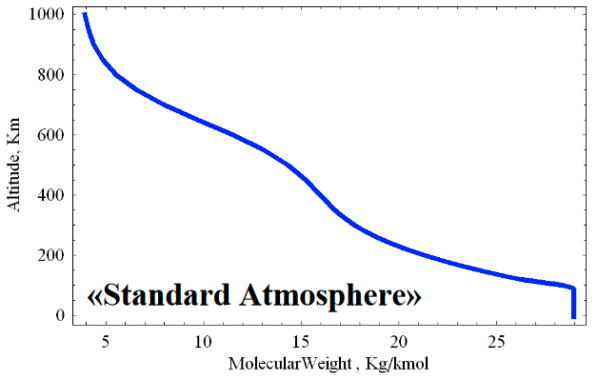
\includegraphics[width=0.5\textwidth]{images/mu(z).png}
\caption{Зависимость среднего молекулярного веса воздуха от высоты \cite{Nosov2019-3}.}\label{fig:mu(z)}
\end{figure}

\begin{figure}[!ht]
\centering
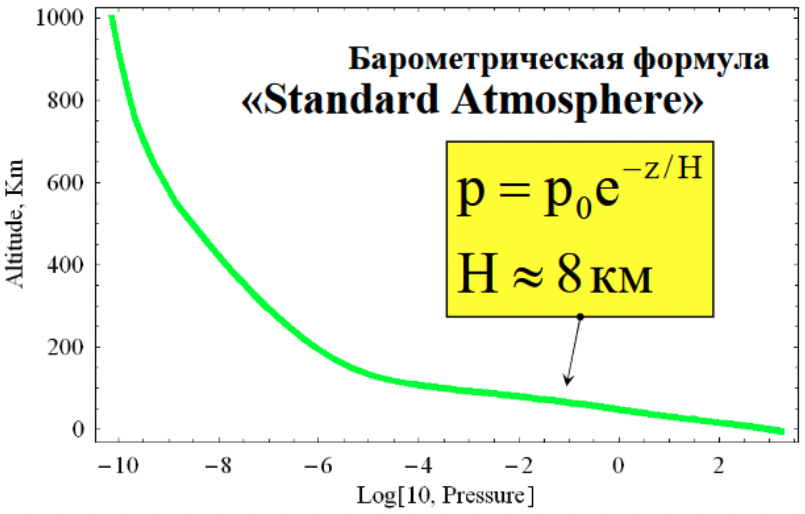
\includegraphics[width=0.5\textwidth]{images/P(z).png}
\caption{Зависимость давления воздуха от высоты \cite{Nosov2019-3}.}\label{fig:P(z)}
\end{figure}

С точки зрения распределения температуры воздуха по высоте выделяют следующие области атмосферы (см. рис. \ref{fig:T(z)}):
\begin{enumerate}
\item Тропосфера (0 -- 10 км). Температура убывает примерно 6.5 град/км.
\item Тропопауза. Переходный слой, в котором наблюдается минимум температуры.
\item Стратосфера (до 50 км). Температура повышается из-за поглощения УФ излучения озоном.
\item Стратопауза. Переходный слой, в котором наблюдается максимум температуры.
\item Мезосфера (до 80 км). Снова происходит падение температуры.
\item Мезопауза. Переходный слой, в котором наблюдается минимум температуры.
\item Термосфера. Температура повышается из-за поглощения коротковолнового излучения.
\end{enumerate}

\begin{figure}[!ht]
\centering
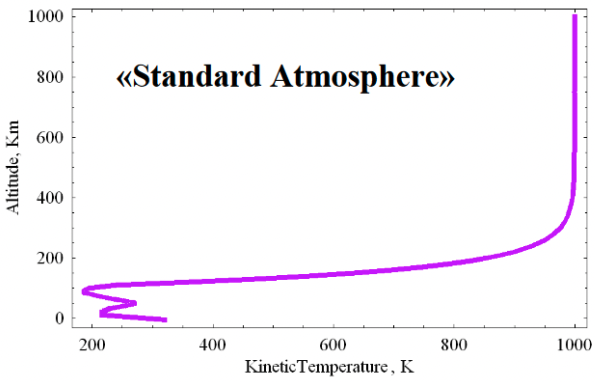
\includegraphics[width=0.5\textwidth]{images/T(z).png}
\caption{Зависимость температуры воздуха от высоты \cite{Nosov2019-3}. Напоминает перевернутую набок греческую букву $\mu$.}\label{fig:T(z)}
\end{figure}
